% Chapter 2

\chapter{Planeaci\'on del producto} % Main chapter title

\label{Chapter2} % For referencing the chapter elsewhere, use \ref{Chapter1} 

%----------------------------------------------------------------------------------------

% Define some commands to keep the formatting separated from the content 

%----------------------------------------------------------------------------------------

\section{Mercado}
El proceso de planeaci\'on empieza con una identificaci\'on de oportunidades para el desarrollo de un producto. Estas oportunidades pueden abarcar cualquiera de los cuatro tipos de proyectos que se describen a continuaci\'on.\\

Los proyectos de desarrollo de productos se pueden clasificar en:

\begin{itemize}
	\item Nuevas plataformas de productos: Este tipo de proyecto comprende un gran esfuerzo de desarrollo para crear una nueva familia de productos basados en una plataforma com\'un. La familia del nuevo producto abordar\'ia mercados y categor\'ias de productos ya conocidos.
	\item Derivados de productos existente: Estos proyectos ampl\'ian una plataforma de productos ya existentes para satisfacer mejor los mercados conocidos con uno o m\'as productos nuevos. 
	\item Mejoras incrementales a productos existentes: En estos proyectos solo se agregan o modifican algunas funciones a productos existentes para mantener actualizada y competitiva la l\'inea del producto.
	\item Productos fundamentalmente nuevos: Estos proyectos abarcan tecnolog\'ias radicalmente nuevas de producci\'on o de producto y pueden ayudar a entrar en mercados nuevos y desconocidos. Estos proyectos involucran en forma inherente m\'as riesgo; no obstante, el \'exito a largo plazo de la empresa puede depender de lo que se aprende en estos importantes proyectos.
\end{itemize}

El tipo de proyecto que comprende este documento ser\'a el de mejoras incrementales a productos existentes, una vez identificado este segmento se realiz\'o la revisi\'on a detalle sobre el primer paso del proceso de planeación del producto.

\begin{figure}[th]
	\centering
	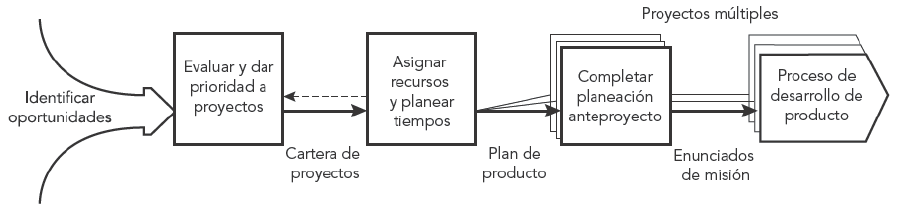
\includegraphics[width=.8\textwidth]{Figures/elproceso.png}
	\decoRule
	\caption{Proceso de planeaci\'on de un producto}
	\label{fig:elproceso}
\end{figure}

\subsubsection{Discapacidad en M\'exico}

De acuerdo con la Clasificaci\'on Internacional del Funcionamiento, de la Discapacidad y de la Salud, presentada en 2001, las personas con discapacidad “son aquellas que tienen una o más deficiencias f\'isicas, mentales, intelectuales o sensoriales y que al interactuar con distintos ambientes del entorno social pueden impedir su participaci\'on plena y efectiva en igualdad de condiciones a las dem\'as”.

Al año 2010, las personas en M\'exico que tienen alg\'un tipo de discapacidad son 5 millones 739 mil 270, lo que representa 5.1\% de la población total.\\
Una de las dificultades m\'as importantes a nivel nacional es la de caminar o moverse. Que referencia a la dificultad de una persona para moverse, caminar, desplazarse o subir escaleras debido a la falta de toda o una parte de sus piernas; incluye tambi\'en a quienes teniendo sus piernas no tienen movimiento o presentan restricciones para moverse, de tal forma que necesitan ayuda de otras persona, silla de ruedas u otro aparato, como andadera o pierna artificial.

\begin{figure}[th]
	\centering
	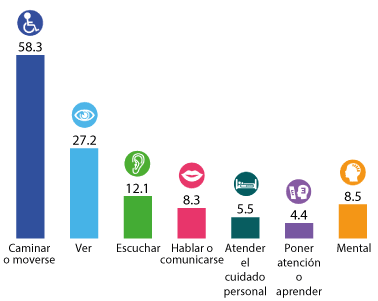
\includegraphics[width=.8\textwidth]{Figures/dificultad.png}
	\decoRule
	\caption{Porcentaje de la poblaci\'on con discapacidad seg\'un dificultad en la actividad (Año 2010)}
	\label{fig:elproceso}
\end{figure}

Algunos otros datos estad\'isticos sobre discapacidad en M\'exico que nos permitir\'an segmentar mejor el mercado para poder ofrecer un producto de valor para la poblaci\'on afectada por esta dificultad son:

\begin{itemize}
\item Las dificultades para caminar y para ver son las m\'as reportadas entre las personas con discapacidad.
\item Los principales detonantes de discapacidad en el pa\'is son las enfermedades (41.3\%) y la edad avanzada (33.1\%).
\item 23.1\% de la poblaci\'on con discapacidad de 15 años y m\'as no cuentan con alg\'un nivel de escolaridad.
\item De la poblaci\'on con discapacidad, 83.3\% es derechohabientes o est\'a afiliada a servicios de salud.
\item Participa en actividades económica 39.1\% de la poblaci\'on con discapacidad de 15 años y más, frente a 64.7\% de su contraparte sin discapacidad
\end{itemize}


\section{Modelo de negocio}

